%The Materials and Methods section provides sufficient detail for other 
%scientists to reproduce the experiments presented in the paper. In some 
%journals, this information is placed in an appendix, because it is not what 
%most readers want to know first.

% explicit preview would be phrased much like the object of the document: 
%"This section first . . . , then . . . , and finally . . . "
% Do not make readers guess: Make sure the paragraph's first sentence gives 
%them a clear idea of what the entire paragraph is about.
%%%%%%%%%%%%%%%%%%%%%%%%%%%%%%%%%%%%%%%%%%%%%%%%%%%%%%%%%%%%%%%%%%%%%%%%%%%%%%
\section{Adaptive Optics Methods applied in Microscopy}
\label{sec:ExperimentDiscussion}

AO has been demonstrated in a range of microscope modalities, including 
conventional widefield microscopes as well as laser scanning systems. The 
most common implementations have involved confocal and two-photon 
fluorescence microscopy, both of which are widely used methods in biomedical 
investigations. Due to aberrations, these microscopes suffer from a 
significant drop in signal and resolution as the focus is moved deeper into 
the specimen. 

Various research groups have combined these microscopes with direct wavefront 
sensing and sensorless AO, normally using deformable mirrors for aberration 
compensation. Ji et al. developed another approach that uses an SLM to 
implement a pupil segmentation phasing method in a two-photon microscope. AO 
has also been applied to microscopes using more exotic contrast mechanisms 
based upon nonlinear optical processes, such as second- and third-harmonic 
generation or coherent anti-Stokes Raman scattering. Using these various 
methods, researchers have demonstrated image improvement at depths of up to 
100 ìm in mouse embryos and over 200 ìm in brain tissue.

Adaptive microscopy is also finding a role in the imaging of live specimens. 
It can help to reduce the time required for image acquisition by increasing 
signal generation and collection efficiency. This is particularly useful in 
microscopes that rely on nonlinear contrast mechanisms, where any drop in 
focal intensity has a compounded effect on signal level.

AO can help by allowing the designer to relax the aberration tolerance from 
the usual fraction of a wavelength up to several wavelengths. This permits a 
significant reduction in the complexity of the optical system. In 
configurations where the optical fidelity has been compromised, the AO can be 
used to correct the residual system aberration, restoring diffractionlimited 
operation.

% explain that we need AO, ref this:
We can conclude: specimen induced aberrations lead to reduced signal levels 
and a deterioration in image quality in optical microscopy, especially in CFM 
and TPM. For the first time, specimen induced aberrations that occur with 
various biological specimens have been classified and quantified for the most 
relevant condition of high NA. The above approach can provide detailed 
information about the variation of each Zernike coefficient across the scan.
As expected from theory, lower NA systems are less susceptible to aberrations 
than high NA system under otherwise similar conditions. Low order correction 
would still provide benefits, even though the initial aberrations are 
smaller. The results presented here quantify the benefit of adaptive optics 
for biological microscopy and provide the bounds within which these systems 
must operate.
\cite{characterizing_abberations}

%%%%%%%%%%%%%%%%%%%%%%%%%%%%%%%%%%%%%%%%%%%%%%%%%%%%%%%%%%%%%%%%%%%%%%%%%%%%%
\subsection{Widefield Microscopy}
\label{sec:WidefieldMicroscopy}

In conventional microscopes, widefield illumination is provided using either 
transmission optics or, in the case of re ection or uorescence modes, via the 
objective lens in an epi configuration. In either case, the image quality 
depends only on the optics of the detection path and is independent of the 
fidelity of the illumination path.
Aberration correction is therefore only necessary in the detection path and a 
single pass adaptive optics system will suffice.
\cite{Aberrations_book} 

\subsubsection{Structured Illumination Microscopy}
\label{sec:StructuredIlluminationMicroscopy}

%next part all from
\cite{wide_AOM_structured_illu}

Optical sectioning microscopy is widely used to provide three-dimensional 
fluorescence images of biological specimens. A common way of obtaining this 
sectioning ability is through point scanning methods such as confocal or 
multiphoton microscopy [1, 2]. An alternative is to use a wide-field 
technique such as structured illumination (SI) microscopy, which retains the 
sectioning ability of confocal microscopy, but can be implemented in a 
conventional microscope using an incoherent light source, and without the 
need for scanning. 

In this technique, the image of a grid is projected on the specimen so as to 
produce a one-dimensional sinusoidal excitation pattern in the focal plane of 
the objective lens. The resulting fluorescence image, consisting of both in-
focus and out-of-focus fluorescence emission, is acquired by a camera. 
Several images are taken, each corresponding to a different grid position. As 
the grid pattern appears only in the focal plane, it is possible to extract 
an optical section from the spatially modulated component of the images via a 
simple calculation.~\cite{wide_structured_illu_principle}.

In this paper we describe wavefront sensorless adaptive optics implemented in 
a SI microscope. It is shown that the final image quality depends 
predominantly on the imaging efficiency of the illumination pattern’s spatial 
frequency. This imaging efficiency is affected much more by some aberration 
modes than by others. Consequently, different aberration modes can have 
significantly different effects on the final sectioned image.

\begin{figure}
	\centering
		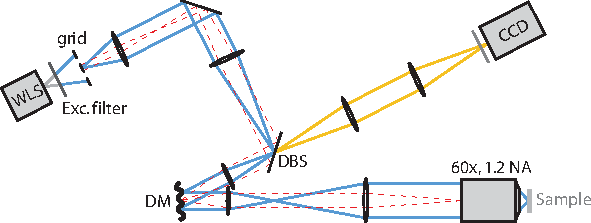
\includegraphics[width=0.75\textwidth]{images/wide_structured_illumination.pdf}
	\caption{Experimental setup for structured illumination microscopy with aberration correction. WLS~-~white light source, DM~-~deformable mirror, DBS~-~dichroic beamsplitter. The blue rays mark the illumination path; the detection path is shown in yellow. Image after~\cite{wide_AOM_structured_illu}.}
	\label{fig:wide_structured_illumination}
\end{figure}

\begin{figure}[tbh]
        \centering
        \begin{subfigure}[b]{0.3\textwidth}
                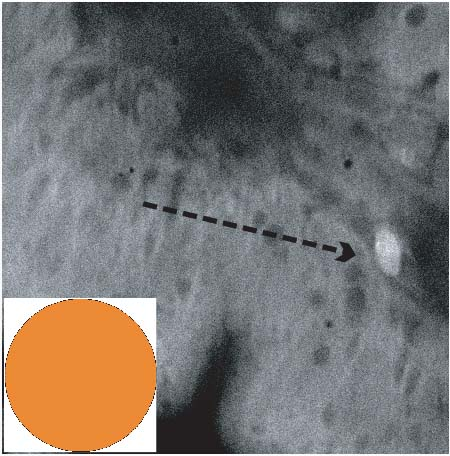
\includegraphics[width=\textwidth]{images/structured_illumination_uncorrected}
                \caption{Reflection.}
                \label{fig:SI_uncorrected}
        \end{subfigure}
        \begin{subfigure}[b]{0.3\textwidth}
                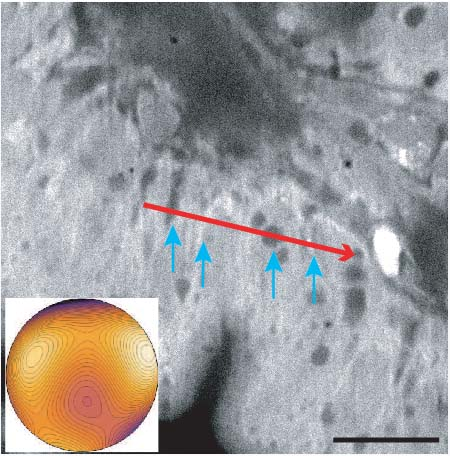
\includegraphics[width=\textwidth]{images/structured_illumination_corrected}
                \caption{Transmission.}
                \label{fig:SI_corrected}
        \end{subfigure}
        \begin{subfigure}[b]{0.3\textwidth}
                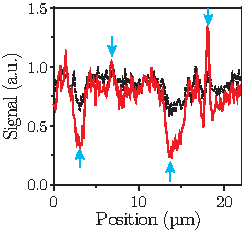
\includegraphics[width=\textwidth]{images/structured_illumination_scan}
                \caption{Transmission.}
                \label{fig:SI_scan}
        \end{subfigure}
								
        \caption{Aberration correction in structured illumination microscopy. A fluorescent mouse intestine sample was imaged (a) without (b) with aberration correction with inserts showing the phase induced by the deformable mirror. (c) Profile along the lines drawn on the images, both profiles normalized so that their mean value is identical. As a result of the resolution improvement, the contrast of small sample features (blue arrows) are better defined after (red solid line) rather than before (black dotted line) correction. The imaging depth was approximately $\unit[10]{\upmu}$, sacle bar size $\unit[10]{\upmu}$. Image after~\cite{wide_AOM_structured_illu}.}
\label{fig:structured_light_correction}
\end{figure} 

\subsubsection{Fluorescence Microscopy}
\label{sec:FlourescnecMicroscopy}

next section, all from \cite{wide_AOM_FM_spehrical_correction} uses a 
standard widefield flourescene microscope but use AOM to correct for 
spherical aberration due to depth -> no specimen induce correction
uses deconvolution to get out of foucs photons corrected

In this paper, we concentrate on the depth dependent aberration which can 
quickly become serious. Imaging 20 mum a live sample (index of refraction 1.36
) with an oil immersion lens causes the peak intensity of the point spread 
function (PSF) to drop 3-fold and the width of the PSF in the axial direction 
to increase by 2-folds. \cite{wide_AOM_FM_spehrical_correction} 

Because wide-field microscopy captures as efficiently as possible every 
emitted photon ultimately minimizing the sample excitation dose, it is well 
suited to in vivo imaging in sampleswhere scattering is not too large. 
Although the out-of-focus photons are in thewrong place, they can be 
effectively re-assigned to the location of emission by constrained 
deconvolution algorithms \cite{wide_deconvolution}

The problem of depth aberrations can be solved by matching the sample index 
and the index of the immersion medium, but this is frequently not feasible or 
desirable. For example, the index of fixed cells can be matched to that of 
the immersion oil, but this option is not available for live imaging.

An important drawback to most schemes that have been proposed so far is that 
they require several images to be taken to optimize the aberration 
correction. This presents a serious problem for live imaging in biology 
because the fluorescence intensities can be weak and susceptible to rapid 
bleaching.

The approach we follow is to correct the depth aberrations withanopen-loop 
predictive algorithm similar totheapproach taken by Potsaid et al. in 
correcting off-axis aberrations. This is possible because the depth 
aberration can be calculated for a given depth into the sample. The depth 
aberration is the result of depth-dependent path length differences.

Correcting depth aberrations with a DM improves both the peak intensities and 
the deconvolution of images taken below the cover slip by removing the depth 
aberration. This allows the use of fast space-invariant deconvolution 
algorithms instead of depth-dependent algorithms. This is significant because 
it improves both the signal-to-noise ratio and the resolution in biological 
imaging where photons are in short supply. Unfortunately, the performance 
does not yet achieve what is theoretically possible.

\begin{figure}[htb]
	\centering
		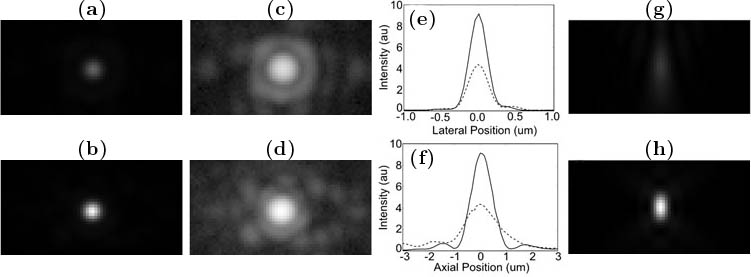
\includegraphics[width=0.80\textwidth]{images/wide_flour_spher_All.jpg}
	\caption{Images of a $\unit[200]{nm}$ bead $\unit[67]{\upmu m}$ below the 
cover slip in a water/glycerol mixture with n = 1.42.  (a) Uncorrected image 
of in-focus plane. (b) Corrected image of in-focus plane. Images (c) and (d) 
are the same as (a) and (b), respectively, but on a logarithmic scale for 
better visualization. (e) and (f) are line profiles of the intensity through 
the center of the bead along the lateral and the longitudinal axis, 
respectively. The dashed line is from the uncorrected image and the solid 
line is from the corrected image. (g) and (h) are simulations of the PSF. 
Images based on \cite{wide_AOM_FM_spehrical_correction}.}
	\label{fig:wide_flour_spher_All} 
\end{figure}


The first is the effect of uncorrected aberrations from the sample and the 
optical path, which decrease the maximum intensity at the cover slip, but in 
a way that does not add linearly to the depth aberration. Thus only a 
fraction of the dispersed photons can be restored to the central peak. In 
closed loop AO systems, system aberrations are automatically compensated at 
each position (Wright et al., 2007), but in an open-loop system this is not 
possible. The second factor is the inability of the mirror to precisely 
conform to the shape given by Eq. (1). The residual error of the mirror shape 
increases with depth (see Fig. 3c) so that as the imaging plane goes deeper 
and the possibility for improvement becomes greater, the improvement in peak 
intensities decreases

Lastly, the ultimate goal of applying adaptive optics in microscopy is to 
correct all aberrations including those introduced by the refractive index 
variations of the sample itself.


\cite{wide_AOM_FM_spehrical_correction}

\cite{wide_MPFM}
\cite{wide_AOM_structured_illu}
\cite{wide_AOM_loew_freq}


%------------------------------------------------------------------------------
-
\subsection{Point Scanning Microscopes}
\label{sec:PointScanningMicroscopes}

Scanning optical microscopes are widely used for high resolution imaging, 
mainly because certain implementations provide three-dimensional resolution 
with optical sectioning and are thus particularly useful for imaging the 
volume structures of biological specimensz. In these microscopes, 
illumination is provided by a laser that is focused by an objective lens into 
the specimen. The light emitted from the specimen is collected, usually 
through the same objective lens, and its intensity is measured by a single 
photodetector. The focal spot is scanned through the specimen in a raster 
pattern and the image is acquired in a point-by-point fashion. The resulting 
data are stored and rendered as images in a computer.

Several other point scanning microscope modalities have been introduced, 
including two-photon excitation uorescence (TPEF) microscopy, second harmonic 
generation (SHG) and third harmonic generation (THG) microscopy, and coherent 
anti-Stokes Raman (CARS) microscopy.

%------------------------------------------------------------------------------
-
\subsubsection{Confocal Microscopes}
\label{sec:ConfocalMicroscopes}

The most common example of this type is the confocal microscope, which can be 
operated in reflection or fluorescence mode. Three-dimensional resolution is 
achieved by the placement of a pinhole in front of the photodetector. In a 
reflection mode confocal microscope, the illumination is scattered by objects 
not only in the focal region, but throughout the focusing cone. In 
fluorescence mode, emission is generated in the focus but also in out-of-
focus regions. The pinhole ensures that mainly light from the focal region 
falls upon the detector and light from out-of-focus planes is obscured. It is 
critical in the confocal microscope that both the illumination and detection 
paths are diffraction limited. This ensures that i) the illuminating focal 
spot is as small as possible, and ii) that the focus is perfectly imaged on 
to the detector pinhole. Therefore, in an adaptive confocal microscope, 
aberration correction must be included in both paths. This dual pass adaptive 
system can usually be implemented using a single deformable mirror, if the 
path length aberrations are the same for both the illumination and the 
emission light. This is the case if there is no significant dispersion in the 
specimen or chromatic aberration in the optics.

A pinhole is not required to obtain three-dimensional resolution, so most 
TPEF microscopes use large area detectors to maximise signal collection. 
Although they rely upon other physical processes, non-linear imaging 
modalities such as SHG, THG and CARS exhibit similar resolution properties. 
When using large area detectors, the fidelity of imaging in the detection 
path is unimportant so the effects of any aberrations in this path are 
negated. It follows that single pass adaptive optics is appropriate for these 
microscopes as aberration correction need only be implemented in the 
illumination path.

Adaptive optics systems have been successfully combined with several point-
scanning microscope systems including confocal,13 TPEF,6, 14, 15 harmonic 
generation,16, 17 CARS.18 Example images of aberration correction in an 
adaptive THG microscope are shown in Fig. 10.

\cite{book_confocal}
\cite{AOM_scan_CFM}


%------------------------------------------------------------------------------
-
\subsubsection{Two-Photon Fluorescence Microscopy}
\label{sec:twoPhotonExcitation}

\cite{TPFM_gated_wavefront}
\cite{TPFM_image_based}
\cite{TPFM_pratical}

%------------------------------------------------------------------------------
-
\subsubsection{Harmonic Generation}
\label{sec:HarmonicGeneration}

\cite{HG_embryos}
\cite{HG_dynamic}


%------------------------------------------------------------------------------
-
\subsubsection{CARS}
\label{sec:CARS}

\cite{CARS}



